\documentclass{beamer}

\usefonttheme{structurebold}

\usepackage[utf8]{inputenc}
\usepackage[T1]{fontenc}
\usepackage[portuguese]{babel} 



\title{Introdução ao \LaTeX}
\date{\today}
\author{Ricardo Peixoto Robaina \\ Tchelinux Bagé}
\institute{Universidade Federal do Pampa}

\usetheme{unipampa}




\begin{document}
	
	\begin{frame}[noframenumbering]
		\titlepage
		\thispagestyle{empty}
	\end{frame}
	
	\begin{frame}{Sumário}
		\setbeamertemplate{section in toc}[sections numbered]
		\tableofcontents[hideallsubsections]
	\end{frame}

\section{Introdução}
\begin{frame}{Introdução}
	
	
	O \LaTeX é um sistema de preparação de documentos com alta qualidade tipográfica.

	
	Grande utilização na escrita de textos técnicos e científicos.
	
	
	O autor preocupa-se com o texto e o \LaTeX\ com a tipografia.
	
	\begin{itemize}
		\item \textbf{TeX} Donald Knuth (1978)  
		\item \textbf{\LaTeX} Leslie Lamport (1983)
	\end{itemize}

\end{frame}

\begin{frame}{Características}
	\begin{itemize}
		\item Tipografia para artigos, relatótios, livros e apresentações de slides
		\item Controle de documentos com referências cruzadas
		\item Tipografia para fórmulas matemáticas
		\item Geração automática de bibliografias
		\item Controle de versão
		%\item Portabilidade
		\item ...
		\item Curva de aprendizagem maior
	\end{itemize}
\end{frame}



\section{Instalação}
\begin{frame}{Instalação}

	\begin{block}{TexLive (Baixa todos os pacotes)}
		\begin{itemize}
			\item sudo apt-get install texlive-full 
		\end{itemize}
	\end{block}
	
	\pause
	
	\begin{block}{MikTeX (Baixa os pacotes sob demanda)}
		\begin{itemize}
			\item https://miktex.org/howto/install-miktex-unx
			
			\item sudo apt-key adv --keyserver hkp://keyserver.ubuntu.com:80 --recv-keys D6BC243565B2087BC3F897C9277A7293F59E4889
			
			\item echo "deb http://miktex.org/download/ubuntu bionic universe" | sudo tee /etc/apt/sources.list.d/miktex.list
			
			\item sudo apt-get update
			
			\item sudo apt-get install miktex
		\end{itemize}
	\end{block}
	

\end{frame}


\begin{frame}{Atualização MikTeX}

	\begin{figure}[!htb]
		\centering
		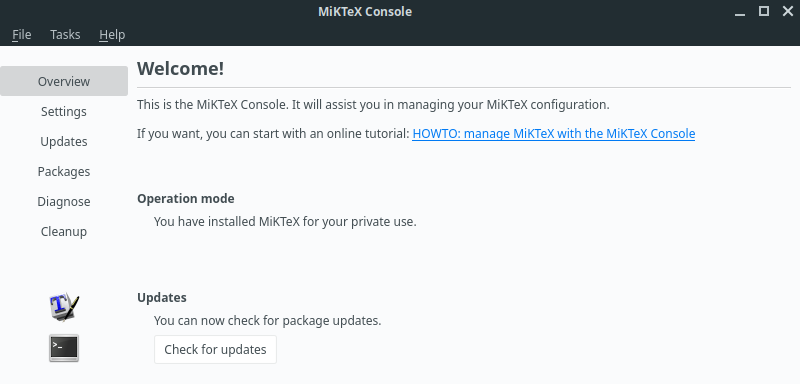
\includegraphics[scale=.38]{miktex.png}
	\end{figure}

\end{frame}

\begin{frame}{Instalação}

	\begin{block}{TexStudio (IDE)}
		\begin{itemize}
			\item sudo apt-get install texstudio
		\end{itemize}
	\end{block}
	
	\pause

	\begin{block}{Resumindo}
		\begin{itemize}
			\item sudo apt-get install texlive-full texstudio 
		\end{itemize}
	\end{block}

\end{frame}


\section{Estrutura dos Documentos}

\begin{frame}{Estrutura}

	\begin{figure}[!htb]
		\centering
		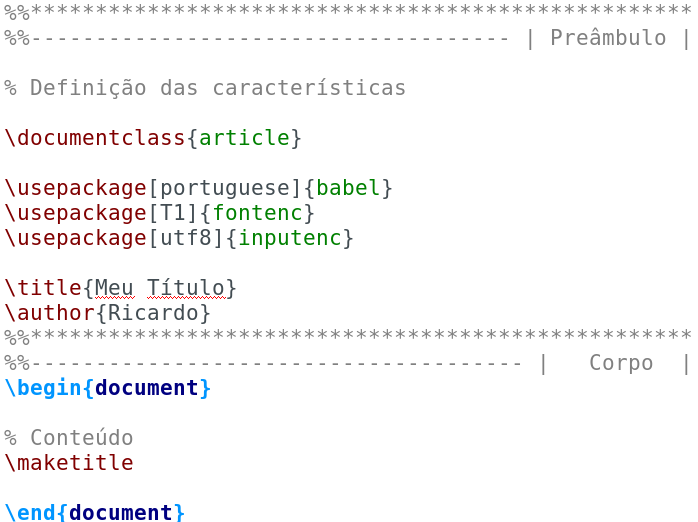
\includegraphics[scale=.4]{estrutura.png}
	\end{figure}

	

\end{frame}




\begin{frame}{Compilação}
	
	\begin{itemize}
		\begin{block}{Criar o arquivo}
			arquivo.tex
		\end{block}
	
		\begin{block}{Compilar}
			pdflatex arquivo.tex
		\end{block}
		
	\end{itemize}

\end{frame}




\section{Criando um Texto}
\begin{frame}{Criando um Texto}

	\begin{itemize}
		\item $\backslash$documentclass\{article\}
		\item $\backslash$documentclass\{book\}
		\item $\backslash$documentclass\{report\}
		\item $\backslash$documentclass\{...\}
	\end{itemize}
	

\end{frame}


\section{Criando um Slide}

	\begin{frame}{Criando um Slide}
	
	\begin{itemize}
		\item $\backslash$documentclass\{beamer\}
	\end{itemize}

\end{frame}

\section{Outras Ferramentas}

\begin{frame}{Outras Ferramentas}
	
	\begin{itemize}
		\item Escrita colaborativa: \textbf{Overleaf} https://v2.overleaf.com \\
		
		\begin{figure}[!htb]
			\centering
			
			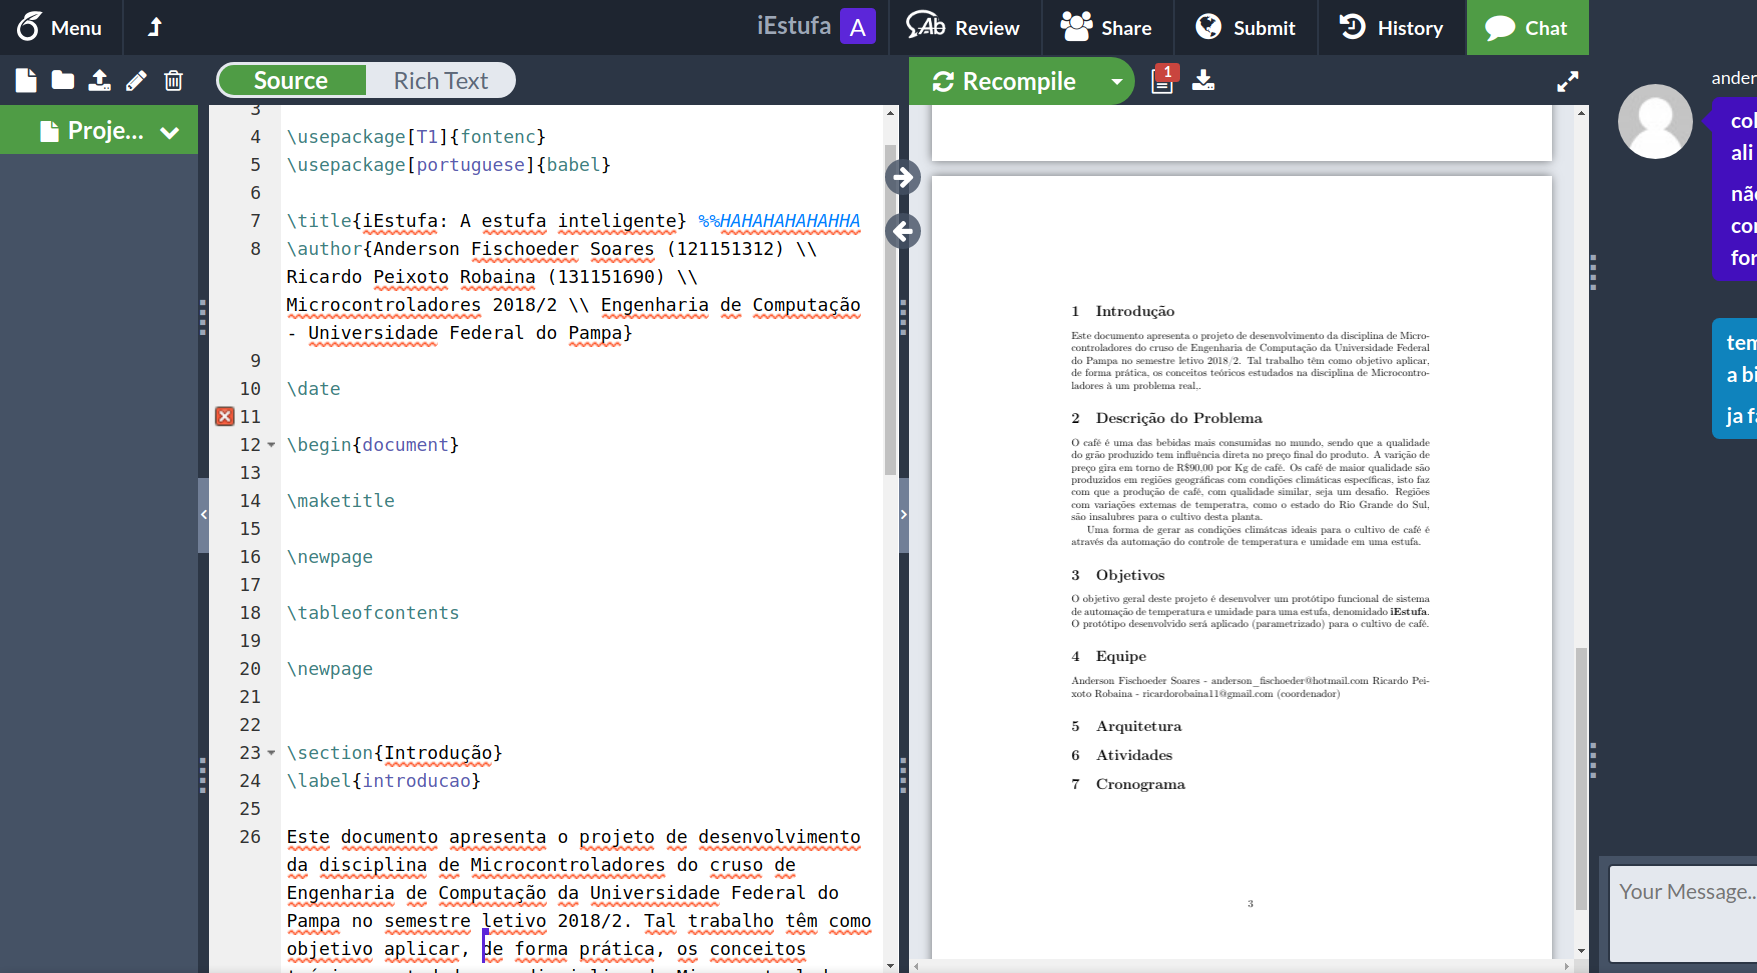
\includegraphics[scale=.15]{ov.png}
		\end{figure}
		
		
		\item Gerenciador de bibliografia: \textbf{JabRef} http://www.jabref.org/
		
	\end{itemize}

\end{frame}

\section{Referências}
	
\begin{frame}{Referências}
	
	
			\begin{itemize}
				\item https://www.latex-project.org/ \\
				
\includegraphics[width=0.5\textwidth]{latex-project-logo.png}
				
				
				\item LaTeX: A Document Preparation System (Leslie Lamport) \\
				
\includegraphics[scale=0.2]{livro.png}
				
			\end{itemize}

	
	
\end{frame}

\begin{frame}{Introdução ao \LaTeX}
	
		\newline
		\begin{center}
			{\Huge  \textbf{Obrigado!} \\}
		\end{center}
		
		{\normalsize 
			\begin{itemize}
				\item ricardorobaina11@gmail.com 
				\item https://github.com/robainaricardo/TchelinuxBage \\ \newline   
			\end{itemize}	
		}
		\maketitle
	
\end{frame}



\end{document}